% 电荷做工
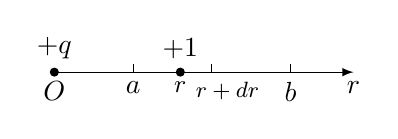
\begin{tikzpicture}[scale=1]
  \draw[-latex] (0,0) -- (3.8,0);
  \node[below] at (3.8,0) {$r$};

  \node[below] at (0,0) {$O$};
  \draw[fill=black] (0,0) circle (0.05cm);
  \node[above] at (0,0.05) {$+q$};

  \draw (1,0) -- (1,0.1);
  \node[below] at (1,0) {$a$};

  \node[below] at (1.6,0) {\small $r$};
  \node[above] at (1.6,0.05) {$+1$};
  \draw[fill=black] (1.6,0) circle (0.05cm);

  \draw (2,0) -- (2,0.1);
  \node[below] at (2.2,0) {\footnotesize $r+dr$};

  \draw (3,0) -- (3,0.1);
  \node[below] at (3,0) {$b$};
\end{tikzpicture}
